\begin{figure}
    \centering
    \begin{subfigure}[b]{0.5\textwidth}
\begin{knitrout}
\definecolor{shadecolor}{rgb}{0.969, 0.969, 0.969}\color{fgcolor}
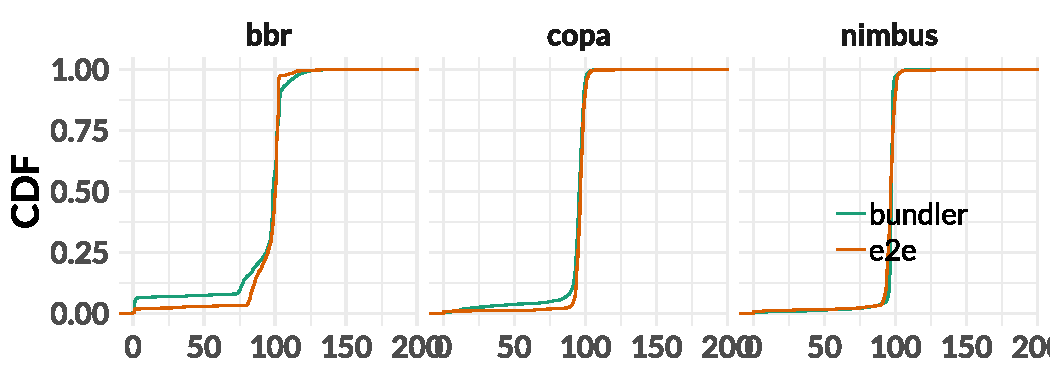
\includegraphics[width=\maxwidth]{figure/eval:tput-delay:a-1} 

\end{knitrout}
    \caption{Throughput (in Mbit/s) Comparison.}\label{fig:eval:tputdelay:a}
    \end{subfigure}
    \begin{subfigure}[b]{0.5\textwidth}
\begin{knitrout}
\definecolor{shadecolor}{rgb}{0.969, 0.969, 0.969}\color{fgcolor}
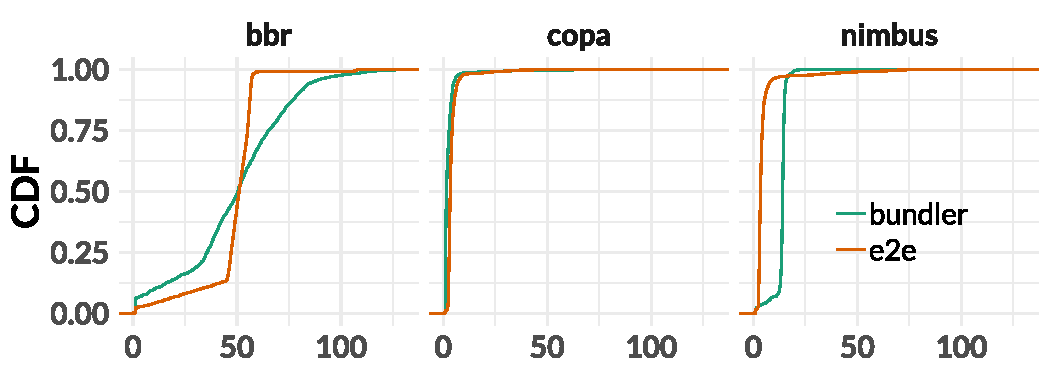
\includegraphics[width=\maxwidth]{figure/eval:tput-delay:b-1} 

\end{knitrout}
    \caption{Delay (in ms) Comparison.}\label{fig:eval:tputdelay:b}
    \end{subfigure}

    \caption{\name can shape underlying Cubic flows so they assume the characteristics of \name's congestion control algorithm.}
    \label{fig:eval:tputdelay}
\end{figure}
